\documentclass{article}
\usepackage{Engineering}
\usetikzlibrary{arrows.meta,calc,patterns,decorations.markings}

\pdftitle{TECHMECH}

\title{\textbf{Technical Mechanics\\HSLU, Semester 2}}
\author{Matteo Frongillo\\(Adapted from \texttt{TECHMECH\_Notes.pdf})}
\date{}

\begin{document}

\maketitle
\tableofcontents
\newpage

%%%%%%%%%%%%%%%%%%%%%%%%%%%%%%%%%%%%%%%%
\section{Static system}
A body of mass $m$ subject to gravity $F_g$ and a normal reaction $F_N$ on a flat surface. In the static case:
\[
\sum F_y = F_N - F_g = 0, 
\quad
\sum F_x = 0
\]

\begin{center}
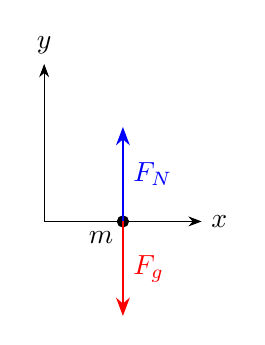
\begin{tikzpicture}[scale=1.0,>=Stealth]
  % Axes
  \draw[->] (0,0) -- (2,0) node[right]{$x$};
  \draw[->] (0,0) -- (0,2) node[above]{$y$};
  % Mass (as a circle)
  \filldraw (1,0) circle (2pt) node[below left]{$m$};
  % Forces
  \draw[->,thick,blue] (1,0) -- (1,1.2) node[midway,right]{$F_N$};
  \draw[->,thick,red]  (1,0) -- (1,-1.2) node[midway,right]{$F_g$};
\end{tikzpicture}
\end{center}

%%%%%%%%%%%%%%%%%%%%%%%%%%%%%%%%%%%%%%%%
\section{Dynamic system}
For a body of mass $m$ under a resultant force $F_{\mathrm{res}}$, the acceleration is 
\[
a = \frac{F_{\mathrm{res}}}{m}
\]

Example with wind $F_w$ acting horizontally and a rope tension or reaction $F_R$:
\[
\sum F_y = 0, 
\quad
\sum F_x = F_w - F_R = 0 \quad (\text{if static in the horizontal direction})
\]

%%%%%%%%%%%%%%%%%%%%%%%%%%%%%%%%%%%%%%%%
\section{Force directions and resultants}
Suppose there are three forces $F_1, F_2, F_3$ in different directions.
\begin{center}
    \begin{tikzpicture}[scale=1.0,>=Stealth]
      % Axes
      \draw[->] (0,0) -- (2.5,0) node[right]{$x$};
      \draw[->] (0,0) -- (0,2.5) node[above]{$y$};
      % F1
      \draw[->,thick,red] (0,0) -- (-1,0) node[midway,above]{$F_1$};
      % F2
      \draw[->,thick,blue] (0,0) -- (1.2,1.2) node[midway,right]{$F_2$};
      % F3
      \draw[->,thick,green!50!black] (0,0) -- (0,-1.4) node[midway,left]{$F_3$};
    \end{tikzpicture}
\end{center}
We can write equilibrium as
\[
\sum F_x = -F_1 + F_2 \cos(\alpha), 
\quad
\sum F_y = -F_3 + F_2 \sin(\alpha)
\]
For instance, if $\alpha = 45^\circ$ and $F_2 = 100\,\mathrm{N}$:
\[
F_1 = F_2 \cos 45^\circ = 70.7\,\mathrm{N}, 
\quad
F_3 = F_2 \sin 45^\circ = 70.7\,\mathrm{N}
\]

%%%%%%%%%%%%%%%%%%%%%%%%%%%%%%%%%%%%%%%%
\section{Ropes}
\textbf{Key property:} Ropes can only carry tensile forces, not compressive or bending forces.

\subsection{Static vs. dynamic with wind}
\begin{itemize}
    \item In a static system with a rope supporting a mass $m$, $\sum F_y = 0$, $\sum F_x = 0$
    \item In a dynamic system with wind $F_w$, $\sum F_y = 0$, $\sum F_x = F_w$
\end{itemize}

%%%%%%%%%%%%%%%%%%%%%%%%%%%%%%%%%%%%%%%%
\section{Moments and couples}
\subsection{Moment}
Moment (torque) is created by a force acting at a distance from a pivot (or reference point):
\[
M_z = F_x \, d_x \quad \text{or} \quad M_z = F_y \, d_y.
\]

\subsection{Couple}
Couple is formed by two equal and opposite forces whose lines of action do not coincide, creating a pure moment.

\begin{center}
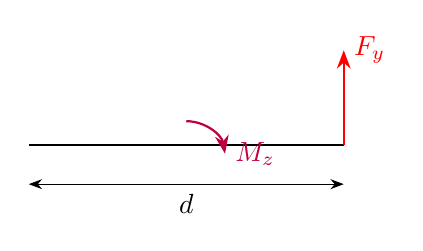
\begin{tikzpicture}[scale=1.0,>=Stealth]
  % Horizontal bar
  \draw[thick] (0,0) -- (4,0);
  % Force at the right
  \draw[->,thick,red] (4,0) -- (4,1.2) node[right]{$F_y$};
  % Distance
  \draw[<->] (0,-0.5) -- (4,-0.5) node[midway,below]{$d$};
  % Show moment arrow
  \draw[->,purple,thick] (2,0.3) arc (90:10:0.5) node[right]{$M_z$};
\end{tikzpicture}
\end{center}

%%%%%%%%%%%%%%%%%%%%%%%%%%%%%%%%%%%%%%%%
\section{Free Body Diagram (FBD)}
\textbf{Procedure:}
\begin{itemize}
\item Isolate the body from its surroundings.
\item Replace each support or contact with the appropriate reaction forces (and possibly moments).
\item Apply equilibrium equations:
  \[
  \sum F_x = 0, 
  \quad
  \sum F_y = 0, 
  \quad
  \sum M = 0.
  \]
\end{itemize}

\begin{center}
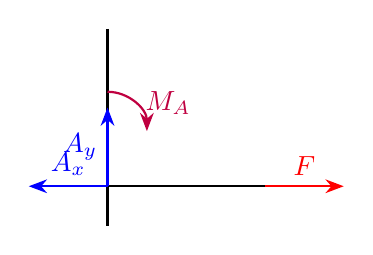
\begin{tikzpicture}[scale=1.0,>=Stealth]
  % Wall
  \draw[thick] (0,2) -- (0,-0.5);
  % Body
  \draw[thick] (0,0) -- (2,0);
  % Force
  \draw[->,thick,red] (2,0) -- (3,0) node[midway,above]{$F$};
  % Reaction at the wall
  \draw[->,thick,blue] (0,0) -- (-1,0) node[midway,above]{$A_x$};
  \draw[->,thick,blue] (0,0) -- (0,1) node[midway,left]{$A_y$};
  % Possibly a moment at the wall
  \draw[->,thick,purple] (0,1.2) arc (90:0:0.5) node[midway,right]{$M_A$};
\end{tikzpicture}
\end{center}

%%%%%%%%%%%%%%%%%%%%%%%%%%%%%%%%%%%%%%%%
\section{Supports}
Every blocked degree of freedom (DOF) introduces a reaction (either a force or a moment). 
In 2D, each point can have up to 3 DOFs:
\[
\text{(1) Translation in } x, \quad
\text{(2) Translation in } y, \quad
\text{(3) Rotation about } z.
\]
\textbf{Types of supports:}
\begin{itemize}
\item \emph{Pin/Hinge}: Fixes $x$ and $y$, allows rotation. (Reactions: $A_x, A_y$)
\item \emph{Roller}: Often fixes $y$ but allows translation in $x$ and rotation. (Reaction: $A_y$)
\item \emph{Fixed/Wall support}: Fixes $x, y$, and rotation. (Reactions: $A_x, A_y, M_A$)
\end{itemize}

%%%%%%%%%%%%%%%%%%%%%%%%%%%%%%%%%%%%%%%%
\section{Examples of Beams or Shelves}
(1) Simply supported beam with two pinned supports.  
(2) Cantilever with a fixed end and free end.  
(3) Beam with supports used for bending tests or balance boards.

\textbf{Small FBD Exercises:}
\begin{itemize}
\item (a) Two vertical forces $F$ at different points, sum up in $y$-direction, etc.
\item (b) Two horizontal forces, $\sum F_x = 2F$, $\sum M = 0$, etc.
\item (c) Summation of vertical forces $F_1 + F_2 = 2F$, etc.
\item (d) Force at $135^\circ$ from horizontal, decompose into $F_x$ and $F_y$, check moments.
\end{itemize}

%%%%%%%%%%%%%%%%%%%%%%%%%%%%%%%%%%%%%%%%
\section{Multi-Body Systems}
Sometimes we have multiple bodies connected at joints, each with its own free-body diagram.

\subsection*{Example}
Let $F = 2000\,\mathrm{N}$, $a = 7\,\mathrm{m}$, $b = 2\,\mathrm{m}$, $c = 6\,\mathrm{m}$, $d = 3\,\mathrm{m}$.  

\begin{enumerate}
\item Draw the FBD of the entire system.  
\item Write equilibrium equations for the unknown reactions $F(A_x)$, $F(A_y)$, $F(B_x)$, $F(B_y)$, etc.  
\item Solve for magnitudes and directions.  
\item Calculate internal forces at the joints if needed.
\end{enumerate}

%%%%%%%%%%%%%%%%%%%%%%%%%%%%%%%%%%%%%%%%
\section{Constraints and Statical Determinacy}
\begin{itemize}
\item \textbf{Statically determinate}: Number of independent equilibrium equations $=$ number of unknowns.  
\item \textbf{Statically indeterminate}: Equations $<$ unknowns.  
\item \textbf{Statically overdeterminate}: Equations $>$ unknowns.
\end{itemize}

\textbf{Examples:}
\begin{itemize}
\item A table with 4 legs on rollers (4 legs $\times$ 3\,DOF each $=12$ unknowns, but only 3 equilibrium equations in 2D) $\Rightarrow$ statically indeterminate.
\item A rod supported by a hinge and a rope (3 unknowns total, 3 equations in 2D) $\Rightarrow$ statically determinate.
\item A rod fixed on both ends (6 unknowns, but only 3 equations in 2D) $\Rightarrow$ statically indeterminate.
\item A shoe on the ground without slipping (3\,DOF, 2 unknowns, friction plus normal) $\Rightarrow$ possibly overdeterminate if friction is large, etc.
\end{itemize}

%%%%%%%%%%%%%%%%%%%%%%%%%%%%%%%%%%%%%%%%
\section{Internal Forces}
To find internal forces (normal, shear, bending moment, etc.), we can make a virtual cut and apply equilibrium to one side of the cut:
\[
N = \text{internal normal force},\quad
Q = \text{internal shear force},\quad
M = \text{bending moment}.
\]

%%%%%%%%%%%%%%%%%%%%%%%%%%%%%%%%%%%%%%%%
\section{Shear/Moment/Tension Diagrams}
\textbf{Procedure:}
\begin{enumerate}
\item Draw the overall FBD, solve for external support reactions.
\item ``Cut'' the beam (or member) at various sections $x$ and solve for the internal forces/moments at each cut to plot $N(x)$, $Q(x)$, $M(x)$.
\end{enumerate}

%%%%%%%%%%%%%%%%%%%%%%%%%%%%%%%%%%%%%%%%
\section{Stress and Bending}
\textbf{Stress} ($\sigma$) is needed to evaluate safety. It differs for each load case:
\[
\sigma_{\text{tensile}} = \frac{F_{\text{int}}}{A}, 
\quad
\sigma_{\text{compressive}} \text{(same formula, different sign)},
\quad
\tau_{\text{shear}} = \frac{F_{\text{shear}}}{A}.
\]
\textbf{Bending} combines tensile, compressive, and possibly shear stress across a cross-section.

\textbf{Strain} ($\varepsilon$) is the internal shape change:
\[
\varepsilon_{\text{tensile}} = \frac{\Delta l}{l_0}, 
\quad
\varepsilon_{\text{compressive}} = \frac{\Delta l}{l_0}, 
\quad
\gamma_{\text{shear}} = \frac{\Delta s}{\Delta h}.
\]
\[
\sigma = E\,\varepsilon,
\]
where $E$ is Young's modulus (in MPa or GPa).

%%%%%%%%%%%%%%%%%%%%%%%%%%%%%%%%%%%%%%%%
\section{Some Young's Modulus Values}
\[
E_{\text{steel}} \approx 210{,}000\,\mathrm{MPa} = 210\,\mathrm{GPa}, \quad
E_{\text{aluminium}} \approx 68{,}000\,\mathrm{MPa} = 68\,\mathrm{GPa}, \quad
E_{\text{polymer}} \approx 2{,}100\,\mathrm{MPa} = 2.1\,\mathrm{GPa}.
\]

\section{Safety Calculation}
A common requirement is:
\[
\sigma_{\text{int}} < \sigma_{\max,\text{admissible}}, 
\quad
\varepsilon_{\text{int}} < \varepsilon_{\max,\text{admissible}},
\]
where allowable (admissible) stresses and strains come from material data and/or a chosen safety factor.

\end{document}